
\documentclass[a4paper,10pt,fleqn, twocolumn]{IEEETran}
\usepackage{amsfonts}
\usepackage{amsthm}
\usepackage{graphicx}
\usepackage{fancyhdr}

\newtheorem{Prop}{Proposition}
\newtheorem{lemma}{Lemma}


\setlength{\parindent}{3em} \setlength{\oddsidemargin}{0in}
\setlength{\textwidth}{6.5in} % sets 1in left and right margins
\setlength{\topmargin}{0.20in} % change to 0.2in for regular latex
%\setlength{\headheight}{0in}
%\setlength{\footheight}{0.5in}
\setlength{\footskip}{0.5in}
\setlength{\textheight}{9.0in} %sets 1in top and bottom margins
\renewcommand{\baselinestretch}{1} %set to 1.5 for double spacing.

\newcommand{\br}{{\mathbf r}}
\newcommand{\bA}{{\mathbf A}}
\newcommand{\ba}{{\bf a}}
\newcommand{\bb}{{\bf b}}
\newcommand{\bc}{{\bf c}}
\newcommand{\bC}{{\bf C}}
\newcommand{\bg}{{\bf g}}
\newcommand{\bG}{{\bf G}}
\newcommand{\bd}{{\bf d}}
\newcommand{\be}{{\bf e}}
\newcommand{\bq}{{\bf q}}
\newcommand{\bs}{{\bf s}}
\newcommand{\bm}{{\bf m}}
\newcommand{\bn}{{\bf n}}
\newcommand{\bu}{{\bf u}}
\newcommand{\bv}{{\bf v}}
\newcommand{\bw}{{\bf w}}
\newcommand{\bx}{{\bf x}}
\newcommand{\by}{{\bf y}}
\newcommand{\bz}{{\bf z}}
\newcommand{\bbf}{{\bf f}}
\newcommand{\bE}{{\bf E}}
\newcommand{\bF}{{\bf F}}
\newcommand{\bL}{{\bf L}}
\newcommand{\bM}{{\bf M}}
\newcommand{\bN}{{\bf N}}
\newcommand{\bS}{{\bf S}}
\newcommand{\bT}{{\bf T}}
\newcommand{\bD}{{\bf D}}
\newcommand{\bX}{{\bf X}}
\newcommand{\bP}{{\bf P}}
\newcommand{\bQ}{{\bf Q}}
\newcommand{\bI}{{\bf I}}
\newcommand{\bR}{{\bf R}}
\newcommand{\bU}{{\bf U}}
\newcommand{\bV}{{\bf V}}
\newcommand{\bW}{{\bf W}}
\newcommand{\bY}{{\bf Y}}
\newcommand{\bZ}{{\bf Z}}
\newcommand{\bJ}{{\bf J}}
\newcommand{\bB}{{\bf B}}
\newcommand{\bzero}{{\bf 0}}
\newcommand{\bgamma}{{\mbox {\boldmath $\gamma$}}}
\newcommand{\btheta}{{\mbox {\boldmath $\theta$}}}
\newcommand{\bLambda}{{\mbox {\boldmath $\Lambda$}}}
\newcommand{\bPsi}{{\mbox {\boldmath $\Psi$}}}
\newcommand{\bPhi}{{\mbox {\boldmath $\Phi$}}}
\newcommand{\bcA}{{\mbox {\boldmath ${\cal A}$}}}
\newcommand{\bcB}{{\mbox {\boldmath ${\cal B}$}}}
\newcommand{\bcC}{{\mbox {\boldmath ${\cal C}$}}}
\newcommand{\bcD}{{\mbox {\boldmath ${\cal D}$}}}
\newcommand{\bcF}{{\mbox {\boldmath ${\cal F}$}}}
\newcommand{\bcN}{{\mbox {\boldmath ${\cal N}$}}}
\newcommand{\bcR}{{\mbox {\boldmath ${\cal R}$}}}
\newcommand{\bcS}{{\mbox {\boldmath ${\cal S}$}}}
\newcommand{\bcH}{{\mbox {\boldmath ${\cal H}$}}}
\newcommand{\bcI}{{\mbox {\boldmath ${\cal I}$}}}


\title{Blind Decision Feedback Interference Cancellation}
\author{LGE Mobile Research (LGEMR)\\San Diego, CA 92131}
\date{}
\begin{document}
\maketitle
\begin{abstract}\small
Interference cancellation is one of the multiuser detection
strategies for suppressing multiple access interference effects
and consequently improving system performance. In this paper, a
blind decision feedback interference cancellation framework and as
well as two classes of blind interference cancellers based on
least-square and minimum mean-square error criteria are proposed
for solving the near-far problem in CDMA. Different to traditional
decision-feedback interference cancellers, the proposed framework
is not an implementation or extension of multistage interference
cancellation in one-symbol period. It makes the detection for the
current symbol using several previous outputs. Compared with
existing blind detectors, the proposed interference cancellers
require a minimum number of previously received signals and no
subspace separation or sequence estimation operation. The
computation complexity can therefore be much low and detection
delay is reduced too. Theoretical analysis and computer
simulations are provided to demonstrate the performance of the
proposed schemes. All these can easily be extended for
asynchronous CDMA.
\end{abstract}

\section{Introduction}
Interference cancellation (IC) is the strategy for forming an
estimate of interference, which may be intersymbol interference
(ISI), spatial interference and/or multiple access interference
(MAI), and then subtracting interference estimate from received
signal before detection. Interference cancellation provides a
promising alternative to conventional or optimum multiuser
detectors (MUD) since it typically requires less implementation
complexity while practically offering similar performance.
Compared with other multiuser detection schemes, interference
cancellation focuses more attention on interference estimation and
different interference estimation methods lead to different
interference cancellation schemes~\cite{Verd98,Wang02b}, including
successive cancellation~\cite{Kohno91}, multistage
detection~\cite{Vara88}, decision-feedback interference
cancellation~\cite{Kave85,Duel93,Duel95}, etc.. Decision-feedback
interference cancellation (DF-IC) is the decision-driven detection
scheme that combines several features of successive interference
cancellation and multistage detection. Minimum mean-squared error
(MMSE) decision-feedback detection is due to Kavehrad and
Salz~\cite{Kave85}. The decorrelating decision-feedback detectors
were firstly proposed by Duel-Hallen~\cite{Duel93,Duel95}.  Recent
research has been devoted to blind implementation of interference
cancellation or multiuser
detection~\cite{Madh94,Wang98,Wang99B,Zhang02} for practical
applications, where only desired users' signal signatures are
available. For most blind implementations, adaptive filter
techniques, e.g., Wiener filters~\cite{Madh94} or Kalman
filters~\cite{Zhang02} techniques, and signal spectrum estimation
techniques~\cite{Wang98,Wang99} are among the most popular
approaches. However, the blind detectors based on these approaches
are known to be difficult to be implemented in many practical
situations.

In order to solve the near-far problem using minimum prior
knowledge and computation complexity, we provide an alternative
blind DF-IC design framework, which only needs a small amount of
previously received signals and detection outputs instead of a
large number of previously received signals required by most
existing blind detectors. The received signal here is taken as a
combination of desired user(s)' spreading sequences, several
previously received signals and noise and the interference can be
blindly estimated out using least-square (LS), maximum likelihood
(ML) or MMSE criterion. The proposed framework is simple and only
requires desired user(s)' signatures and timing and also a small
number of previously received signals. There is no converging,
estimation or subspace separation procedure employed by other
blind detectors~\cite{Madh94,Honi95,Wang98,Wang99}. Hence the
complexity and detection delay are much reduced. Theoretical
analysis and computer simulations are finally presented to
demonstrate the performance of these blind detectors. The proposed
framework and approaches can be easily applied for asynchronous
CDMA channels.

\section{System Model And Problem Description}
We consider forward-link transmissions in a single-cell DS/CDMA
system. There are $K$ active users over the multipath channel with
$P$ strong paths~\footnote{Strong paths are those to be explicitly
combined by RAKE receiver.} and the channel is an additive white
Gaussian noise (AWGN) channel. The baseband representation of the
received signal due to user $k$ is given by
\begin{equation}
\begin{array}{rcl}
r_k(t)&=&\sum\limits_{p=1}^{P}\alpha_{pk}A_k[n]
b_k[n]c_k(t-nT-\tau_p)
\end{array}
\end{equation}
\noindent where $\alpha_{pk}$ is the $p$th path loss of user $k$'s
signal, $b_k{[n]}$ is the $n$th bit sent by user $k$. We assume
that the $\left\{b_k{[n]}\right\}$ are independent and identically
distributed random variables with $E\left\{b_k{[i]}\right\}=0$ and
$E\left\{|b_k{[i]}|^2\right\}=1$. The parameters $c_k(t)$ denote
the normalized spreading signal waveform of user $k$ during the
interval $[0,\ T]$, $\tau_1\leq\tau_2\leq\ldots\leq\tau_P$,
denotes $P$ different transmission delays from the base station to
user $k$ and $A_k[n]$ is the amplitude of the received signal for
user $k$ at time $t=n$. The total baseband signal received by user
$k$ is
\begin{equation}
\begin{array}{rcl}
\tilde{r}(t)&=&\sum\limits_{k=1}^{K}r_k(t)
\end{array}
\end{equation}
The received signal $\tilde{r}(t)$ is passed through the
corresponding chip matched filter (CMF) $\phi(t)$ and RAKE
combiner. The combined output $r(t)$ is~\footnote{Without loss of
the generality, we drop the time index $n$ in the following
discussion.}
\begin{equation}\hspace{-0.0in}
\begin{array}{rcl}
r(t)&=&A_k b_k c_k(t-nT-\tau_1)\otimes \phi(t-\tau_1)+ \\
&&\hspace{0.0in} m_{\rm ISI}(t) + m_{\rm MAI}(t) + n(t)
\end{array}\label{r_t}
\end{equation}
\noindent where
\begin{equation} \hspace{-0.05in}
\begin{array}{rcl}
 m_{\rm ISI}(t)&=&\\
 &&\hspace{-0.83in}\sum\limits^{P}_{p\neq
q}\beta_{qk} \alpha_{pk}A_kb_kc_k(t-nT+\tau_{q1}-\tau_1)\otimes
\phi(t-\tau_1)
\end{array}
\end{equation}
\noindent is the intersymbol interference (ISI) to user $k$,
\begin{equation} \hspace{-0.17in}
\begin{array}{rcl}
m_{\rm MAI}(t)&=&\sum\limits_{i\neq
 k}^{K}A_ib_ic_i(t-nT-\tau_1)\otimes\phi(t-\tau_1)+\\
 &&\hspace{-0.75in}\sum\limits_{i\neq
 k}^{K}\sum\limits^{P}_{p\neq
q}\beta_{qk}
\alpha_{pi}A_ib_ic_i(t-nT+\tau_{q1}-\tau_p)\otimes\phi(t-\tau_1)
\end{array}
\end{equation}
\noindent is the MAI to user $k$, $\beta_{qk}$ is the weight of
the $q$th RAKE finger with
$\sum\limits_{q=1}^{P}\beta_{qk}\alpha_{qk}=1$ and $\tau_{q1} =
\tau_{q}-\tau_1$ is the propagation delay difference between the
$1$st path and $p$th path. $\otimes$ denotes the convolutional
product. $n(t)$ is AWGN with variance $\sigma^2$. The user $k$'s
RAKE output can be sampled at $f_s=1/T_s$ and straightforwardly
expressed by
\begin{equation}\hspace{-0.1in}
\begin{array}{rcl}
\br&=&\left[
\matrix{r(nT+T_s+\tau_1)&\ldots&r(nT+LT_s+\tau_1)}\right]^{\rm
T}\\
 &=&\sum\limits_{k=1}^{K} A_k b_k \bs_k + \bn \\
 &=&\bS \bA \bb + \bn
\end{array}\label{r_sync}
\end{equation}
\noindent where $\bS=[\bs_1\ \bs_2\ \ldots\ \bs_K]$ is the
received spreading sequence matrix combined with both ISI and MAI
information, and $L=T/T_s$ is the number of samples per symbol,
which usually is not less than the spreading gain $L_c$.

Because of $m_{\rm MAI}(t)$ existing in the received signal
$r(t)$, the performance of conventional matched filter receiver
suffers from the so-called near-far problem~\cite{Verd98}.
Interference cancellation is one of the receiver techniques for
solving this problem.

\section{Blind Interference Cancellation}
\begin{figure} \center{
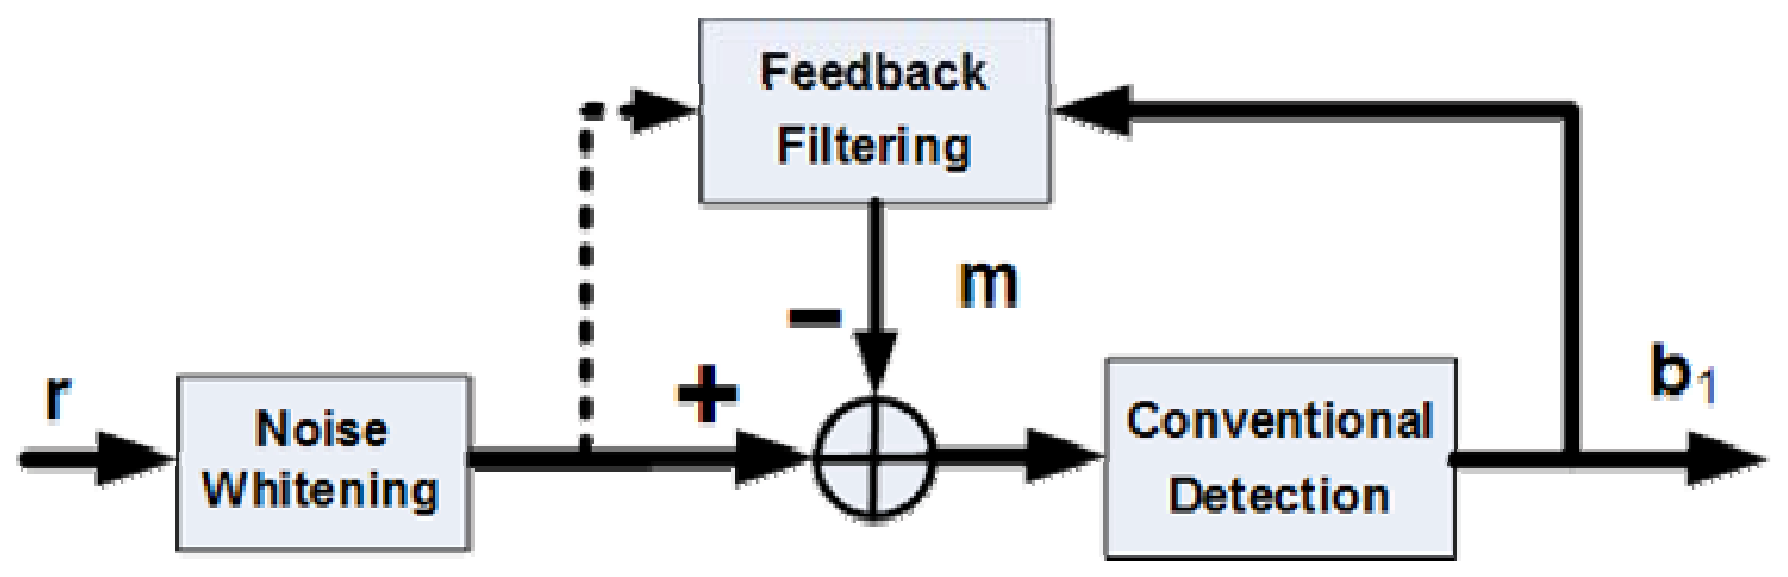
\includegraphics[width=3.2in]{BDFIC1.eps}
\caption{A group-wised decision feedback interference cancellation
block diagram} }\label{DFIC}
\end{figure}
Without loss of the generality, only the signals for the first $G$
desired users are detected and their spreading signatures
$\bS_1=\left[\matrix{\bs_1&\bs_2&\ldots&\bs_G}\right]$ are known
beforehand. In order to blindly estimate MAI without knowing the
original spreading matrix $\bS$, we define a blind MAI signature
matrix
\begin{equation}
\begin{array}{rcl}
\bcS&=&\bigl[\matrix{{\br}[n-1]&{\br}[n-2]&\ldots&{\br}[n-M]}\bigr]\\
&=&\bS\bA\bB+\bN\\
&=&\bS_1\bA_1\bB_1+\bS_2\bA_2\bB_2+\bN
\end{array} \label{bcs}
\end{equation}
\noindent where $\bar\br[n-m]=\br[n-m]-\bS_1\bA_1\bb_1[n-m]$,
$m=1,\ 2,\ \ldots,\ M$ and $K\leq M+G\leq L$.
$\bB=\bigl[\bB_1^{\rm H}\ \bB_2^{\rm H}\bigr]^{\rm H}$ is the
detected data matrix for $\bcS$, $\bS_2$ is the original spreading
signature for interfering users, $\bA_1$, $\bA_2$, $\bB_1$ and
$\bB_2$ are the amplitude matrices and data matrices for desired
users and interfering users, respectively. $M=K-G$ is the minimum
number for blind interference canceller to unambiguously
distinguish different interfering signals. The relationship
between $\bcS$ and the MAI $\bm$ can be written by
\begin{equation}\hspace{-0.0in}
\begin{array}{rcl}
\bm &=&\bS_2\bA_2\bb_2\\
&=&\bigl(\bcS-\bS_1\bA_1\bB_1-\bN\bigr)\bB_2^{+}\bb_2\\
&=&\bcS\bbf-\bS_1\bD_1\bbf+\tilde{\bn}
\end{array}\label{bm}
\end{equation}
\noindent where $\bbf=\bB_2^{+}\bb_2$ denotes the projection of
$\bm$ onto the column space of $\bS_2\bA_2\bB_2$, which is similar
to $\bS_2$, $\bD_1=\bA_1\bB_1$ and
$\tilde{\bn}=-\bN\bB_2^{+}\bb_2$. With (\ref{bm}), it shows that
$\bm$ can be estimated out if $\bbf$ is known. In order to
estimate $\bbf$, we perform QR-decomposition on $\bS_1$ so that
\begin{equation}
\begin{array}{rcccl}
\bS_1&=&\bQ_1\bR_1&=&\bQ_{11}\bR_{11}
\end{array},
\end{equation}
\noindent where $\bQ_1=\left[\bQ_{11}\
\bQ_{12}\right]\in\mathbb{R}^{L\times L}$ is orthogonal and
$\bR_1=[\bR_{11}^{\rm H}\ \bzero^{\rm H}]^{\rm
H}\in\mathbb{R}^{L\times G}$, and apply $\bQ_{12}^{\rm H}$ on both
sides of (\ref{bm}). We then get
\begin{equation}
\begin{array}{rcl}
\bQ_{12}^{\rm H}\bm&=&\bQ_{12}^{\rm H}\bcS\bbf+\bQ_{12}^{\rm
H}\tilde\bn
\end{array}
\end{equation}
\noindent Since
\begin{equation}\hspace{-0.0in}
\begin{array}{rcl}
\bQ_{12}^{\rm H}\br&=&\bQ_{12}^{\rm H}\bm + \bQ_{12}^{\rm H}\bn
\end{array},
\end{equation}
\noindent $\bbf$ can be estimated from
\begin{equation}\hspace{-0.0in}
\begin{array}{rcl}
\bQ_{12}^{\rm H}\br&=&\bQ_{12}^{\rm H}\bcS\bbf+\bQ_{12}^{\rm
H}\bar\bn
\end{array},\label{f2}
\end{equation}
\noindent where $\bar\bn=\tilde\bn+\bn$. After $\bbf$ is
estimated, the MAI $\bm$ can be estimated from (\ref{bm}) so that
$\bA_1$ and $\bb_1$ can be estimated and detected from
\begin{equation}
\begin{array}{rcl}
\br&=&\bS_1\bA_1\bb_1-\left(\bcS-\bS_1\bD_1\right)\hat{\bbf}+\bar\bn
\end{array}\label{br_bm}
\end{equation}
\noindent where $\hat{\bbf}$ is an estimate of $\bbf$. Since the
previous outputs $\bD_1$ are used for estimating interference
$\bm$ and $\bA_1$ and detecting $\bb_1$ without involving $\bS_2$,
this interference cancellation framework is named blind
decision-feedback interference cancellation.

\subsection{\em Least Square IC}
If $\hat{\bbf}$ is known in least square interference cancellation
approaches, $\hat{\bb}_1$ can be estimated by
\begin{equation}\hspace{-0.09in}
\begin{array}{l}
\hat{\bb}_1=\mbox{arg}\min\limits_{\bx}\left\|\br-\left(\bcS_2-\bS_1\bD_1\right)\hat{\bbf}-\bS_1\hat{\bA}_1\bx\right\|_2.
\end{array}\label{b_LS}
\end{equation}
There are typically two approaches for estimating $\bbf$ with
least square criterion. The first one is the classic least-square
approach, which can be expressed by
\begin{equation}\hspace{-0.00in}
\begin{array}{rcl}
{\bbf}_{\rm LS}&=&\mbox{arg}\min\limits_{\by}\left\|\bQ_{12}^{\rm
H}\br-\bQ_{12}^{\rm H}\bcS\by\right\|_2\\
&=&\bcS^{+}\br
\end{array}
\end{equation}
\noindent and the LS-IC output $\hat\bb_{1\rm LS}$ for the first
$G$ users can then be written by
\begin{equation}\hspace{-0.0in}
\begin{array}{rcl}
\hat{\bb}_{1\rm
LS}&=&\bS_{1}^{+}\br-\bS_{1}^{+}\left(\bcS_{2}-\bS_{1}\bD_1\right)\bcS^{+}\br.
\end{array}\label{b_LS_IC}
\end{equation}

\subsection{\em Total Least Square IC}
\noindent The second is the total-least-square (TLS) approach,
which can be expressed by
\begin{equation}\hspace{-0.07in}
\begin{array}{rcl}
\left[\matrix{\hat{\bZ}\cr{\bbf}_{\rm
TLS}}\right]&=&\mbox{arg}\min\limits_{\bZ\
\by}\left\|\left[\matrix{\bQ_{12}^{\rm H}\bcS\cr\bQ_{12}^{\rm
H}\br}\right]-\left[\matrix{\bZ\cr\bZ\by}\right]\right\|_2
\end{array}.
\end{equation}
\noindent If $\sigma_{K-G}'>\sigma_{K-G+1}$, the TLS estimation of
$\bbf$ is~\cite{Huff91}
\begin{equation}\hspace{-0.070in}
\begin{array}{l}
{\bbf_{\rm TLS}}=\left(\bcS^{\rm H}\bQ_{12}\bQ_{12}^{\rm
H}\bcS-\sigma_{K-G+1}^{2}\bI\right)^{-1}\bcS^{\rm
H}\bQ_{12}\bQ_{12}^{\rm H}\br
\end{array}\label{f_TLS}
\end{equation}
\noindent where $\sigma_{K-G}'$ and $\sigma_{K-G+1}$ are the
$(K-G)$th and $(K-G+1)$th largest singular value of $\bQ_{12}^{\rm
H}\bcS$ and $\bQ_{12}^{\rm H}\left[\matrix{\br&\bcS}\right]$. The
TLS-IC $\hat{\bb}_{1\rm TLS}$ can be expressed by
\begin{equation}\hspace{0.0in}
\begin{array}{rcl}
\hat{\bb}_{1\rm
TLS}&=&\bS_{1}^{+}\br-\bS_{1}^{+}\left({\bcS}_{2}-{\bS}_{1}{\bD_1}\right){\bbf_{\rm
TLS}}
\end{array}\label{b_TLS_IC}
\end{equation}
\subsection{\em Joint Least Square IC}
Furthermore, a joint LS scheme, which combines ($\ref{b_LS}$) and
($\ref{f_TLS}$), can be written by
\begin{equation}\hspace{-0.09in}
\begin{array}{l}
\left[\matrix{{\hat\bb}_{\rm JLS}\cr\bbf_{\rm
JLS}}\right]=\mbox{arg}\min\limits_{\bx}\left\|\br-\left[\bS_1\hat{\bA}_1\
\left(\bcS_2-\bS_1\bD_1\right)\right]\left[\matrix{\bx\cr\hat{\bbf}}\right]\right\|_2.
\end{array}\label{b_LS}
\end{equation}


\subsection{\em Maximum Likelihood IC}
For the linear signal model in (\ref{br_bm}), the maximum
likelihood interference cancellation can be written by
\begin{equation}\hspace{-0.12in}
\begin{array}{rcl}
\hat{\bb}_1&=&\mbox{arg}\min\limits_{\bx}\left\{\mathbf\delta_{\bb_1}^{\rm
H}\bR_{\bar\bn}\mathbf\delta_{\bb_1}\right\},
\end{array}
\end{equation}
\noindent where
\begin{equation}
\begin{array}{rcl}
\mathbf\delta_{\bb_1}&=&\br-\bS_1\bA_1\bx-\left(\bcS-\bS_1\bD_1\right)\hat{\bbf}
\end{array},
\end{equation}
\noindent and $\hat\bbf$ can be estimated with minimizing
\begin{equation}\hspace{-0.00in}
\begin{array}{rcl}
{\bbf}_{\rm
ML}=\mbox{arg}\min\limits_{\by}\left\{\mathbf\delta_{\bbf}^{\rm
H}\bR_{\bar\bn}\mathbf\delta_{\bbf}\right\}
\end{array},
\end{equation}
\noindent where
\begin{equation}\hspace{-0.00in}
\begin{array}{rcl}
\mathbf\delta_{\bbf}&=&\bQ_{12}^{\rm H}\br-\bQ_{12}^{\rm H}\bcS\by
\end{array}.
\end{equation}



\subsection{\em Minimum Mean-Square Error IC}
In MMSE-based approach,the interference cancellation is done with
solving
\begin{equation}\hspace{-0.15in}
\begin{array}{l}
\hat{\bb}_1=\mbox{arg}\min\limits_{\bx}\mbox{E}\left\|\br-\left(\bcS_2-\bS_1\bD_1\right)\hat{\bbf}-\bS_1\hat{\bA}_1\bx\right\|_2
\end{array}
\end{equation}
\noindent providing $\hat{\bbf}$ is known. On the other hand,
$\bbf$ is estimated with minimizing MSE
\begin{equation}\hspace{-0.08in}
\begin{array}{rcl}
{\bbf}_{\rm
MMSE}&=&\mbox{arg}\min\limits_{\bx}\mbox{E}\left\|\bQ_{12}^{\rm
H}\br-\bQ_{12}^{\rm H}\bcS\bx\right\|_2^2\\
&=&\left(\bcS^{\rm H}\bQ_{12}\bQ_{12}^{\rm
H}\bcS-\sigma^{2}\bI\right)^{-1}\bcS^{\rm H}\bQ_{12}\bQ_{12}^{\rm
H}\br
\end{array}
\end{equation}
\noindent so that the MMSE-IC for BPSK modulation can be written
by
\begin{equation}\hspace{-0.10in}
\begin{array}{l}
\hat{\bb}_1=\\
\mbox{sgn}\left\{\left(\bS_1\hat{\bA}_1^2\bS_1^{\rm
H}-\sigma^2\bI\right)^{+}\bS_1^{\rm
H}\left[\br-\left(\bcS_2-\bS_1\bD_1\right){\bbf}_{\rm
MMSE}\right]\right\}.
\end{array}
\end{equation}


\section{Performance Analysis}
\subsection{\em Geometric Explanation}
It is known that conventional decorrelating detection is an
oblique projection of received signals onto desired users' signal
subspace along the interference subspace~\cite{Elda02}. For the
proposed interference cancellation framework, it actually
orthogonally projects received signals, including both the
currently and previously received signal, onto the complementary
orthogonal subspace of desired users' signal subspace and
estimates interference through this projection.

\subsection{\em Relationship with Blind MUD}
It can be proven that the LS-IC in (\ref{b_LS_IC}) actually is
equal to the blind LS decorrelating detector
\begin{equation}
\begin{array}{rcl}
\hat{\bb}_{1}&=&\mbox{sgn}\left\{\left[\matrix{\bI&\bB_1}\right]\bA\bbf_{\rm
LS}\right\}
\end{array}
\end{equation}
\noindent with respect to
\begin{equation}
\begin{array}{rcl}
{\bbf}_{\rm
LS}&=&\matrix{\mbox{arg}\min\limits_{\bx}\left\|\br-\left[\matrix{\bS_1&\bcS}\right]\bx\right\|_2^2}
\end{array}
\label{LSProb}
\end{equation}
\noindent and MMSE-IC is equal to the blind MMSE detector
\begin{equation}\hspace{0.0in}
\begin{array}{rcl}
\hat{\bb}_1&=&\mbox{sgn}\left\{\left[\matrix{\bI&\bB_1}\right]\bA\bbf_{\rm
MMSE}\right\}
\end{array}
\end{equation}
\noindent with respect to
\begin{equation}
\begin{array}{rcl}
{\bbf}_{\rm
MMSE}&=&\mbox{arg}\min\limits_{\bx}\mbox{E}\left\|\br-\left[\matrix{\bS_1&\bcS}\right]\bx\right\|_2^2
\end{array}.
\end{equation}

\subsection{\em AME and Near-Far Resistance}
A commonly used performance measure for a multiuser detector is
asymptotic multiuser efficiency (AME) and near-far
resistance~\cite{Verd98}. Since the proposed algorithms converges
to the conventional decorrelating detector as $\sigma^2\rightarrow
0$, their AME and near-far resistance are identical to the
decorrelating detector:
\begin{equation}
\begin{array}{rcl}
\bar{\eta}_k&=&\frac{1}{\left[\bR^{+}\right]_{kk}}
\end{array}.
\end{equation}
\subsection{\em CRLB for $\bbf$ Estimation}
The Cram\'{e}r-Rao Lower Bound (CRLB) is given by the inverse of
the Fisher information matrix (FIM). Providing the blind spreading
matrix $\bcS$ is known beforehand, we first define the parameter
vector $\mathbf{\phi} = \left[\bar{\sigma}^{2}\ \bbf^{\rm
H}\right]^{\rm H}$, where $\bar{\sigma}^{2}
=(1+\frac{M-G}{M-K})\sigma^{2}$, for computing the FIM
\begin{equation}
\begin{array}{rcl}
{\bI(\mathbf{\phi})} &=& {\rm E} \left\{ \left( \frac{\partial
\ln{\cal L}}{\partial \mathbf{\phi}} \right) \left( \frac{\partial
\ln{\cal L}}{\partial \mathbf{\phi}} \right)^{\rm H} \right\}
\label{fim}
\end{array}
\end{equation}
\noindent where $\ln{\cal L}$ is the log-likelihood function given
by
\begin{equation}
\begin{array}{rcl}
\ln{\cal
L}&=&C-L\ln\bar{\sigma}^2-\frac{1}{2\bar{\sigma}^2}\parallel\mathbf{e}\parallel_2^2
\end{array},\label{logl}
\end{equation}
\noindent $C$ is a constant and
$\mathbf{e}=\bT\bQ_1\br-\bcR_{22}\bbf$. Providing $\bcS$ is known,
the closed-form CRLB expression of $\bbf$ is then given by
\begin{equation}
\begin{array}{rcl}
{\rm CRLB}(\bbf\ |\ \bcS) &
=&(1+\frac{M-G}{M-K})\sigma^{2}(\bcR_{22}^{\rm H}\bcR_{22})^{\rm
+}
\end{array}.\label{CRLB_f}
\end{equation}
\noindent It shows that the accuracy of estimating $\bbf$ may
increase with increasing $M$.

\section{Computer Simulations}
There are $K=10$ users with the group size $G=3$ and the spreading
sequences used in simulations are $64$-chip ($L=64$) random
sequences. In the computer simulations, the previous amplitude
estimation from (\ref{A_estimation}) is directly use for the next
detection without any amplitude filtering. From Subplot (a) in
Fig. 3, it is interesting to see that the performance of the
simplest LS detector has the best performance. From Subplot (b),
it is very impressive to find that the performance of blind LS
detector is very close to the conventional decorrelating detector
whatever how strong the MAI is in our simulations when $M$ is
large enough. We then check the performance of the proposed LS
blind detector against the amplitude estimation errors. From Fig.
4, we can see that the BER of the LS detector basically is
unchanged against amplitude estimation error when SNR is large
enough. From Fig. 5, we can see that the performance of the LS
detector can be better providing $M$ is larger enough. This
confirms (\ref{noise_var_new}), which shows that the variance of
$\bar{\bn}$ decrease with increasing $M$.
\begin{figure} \center{
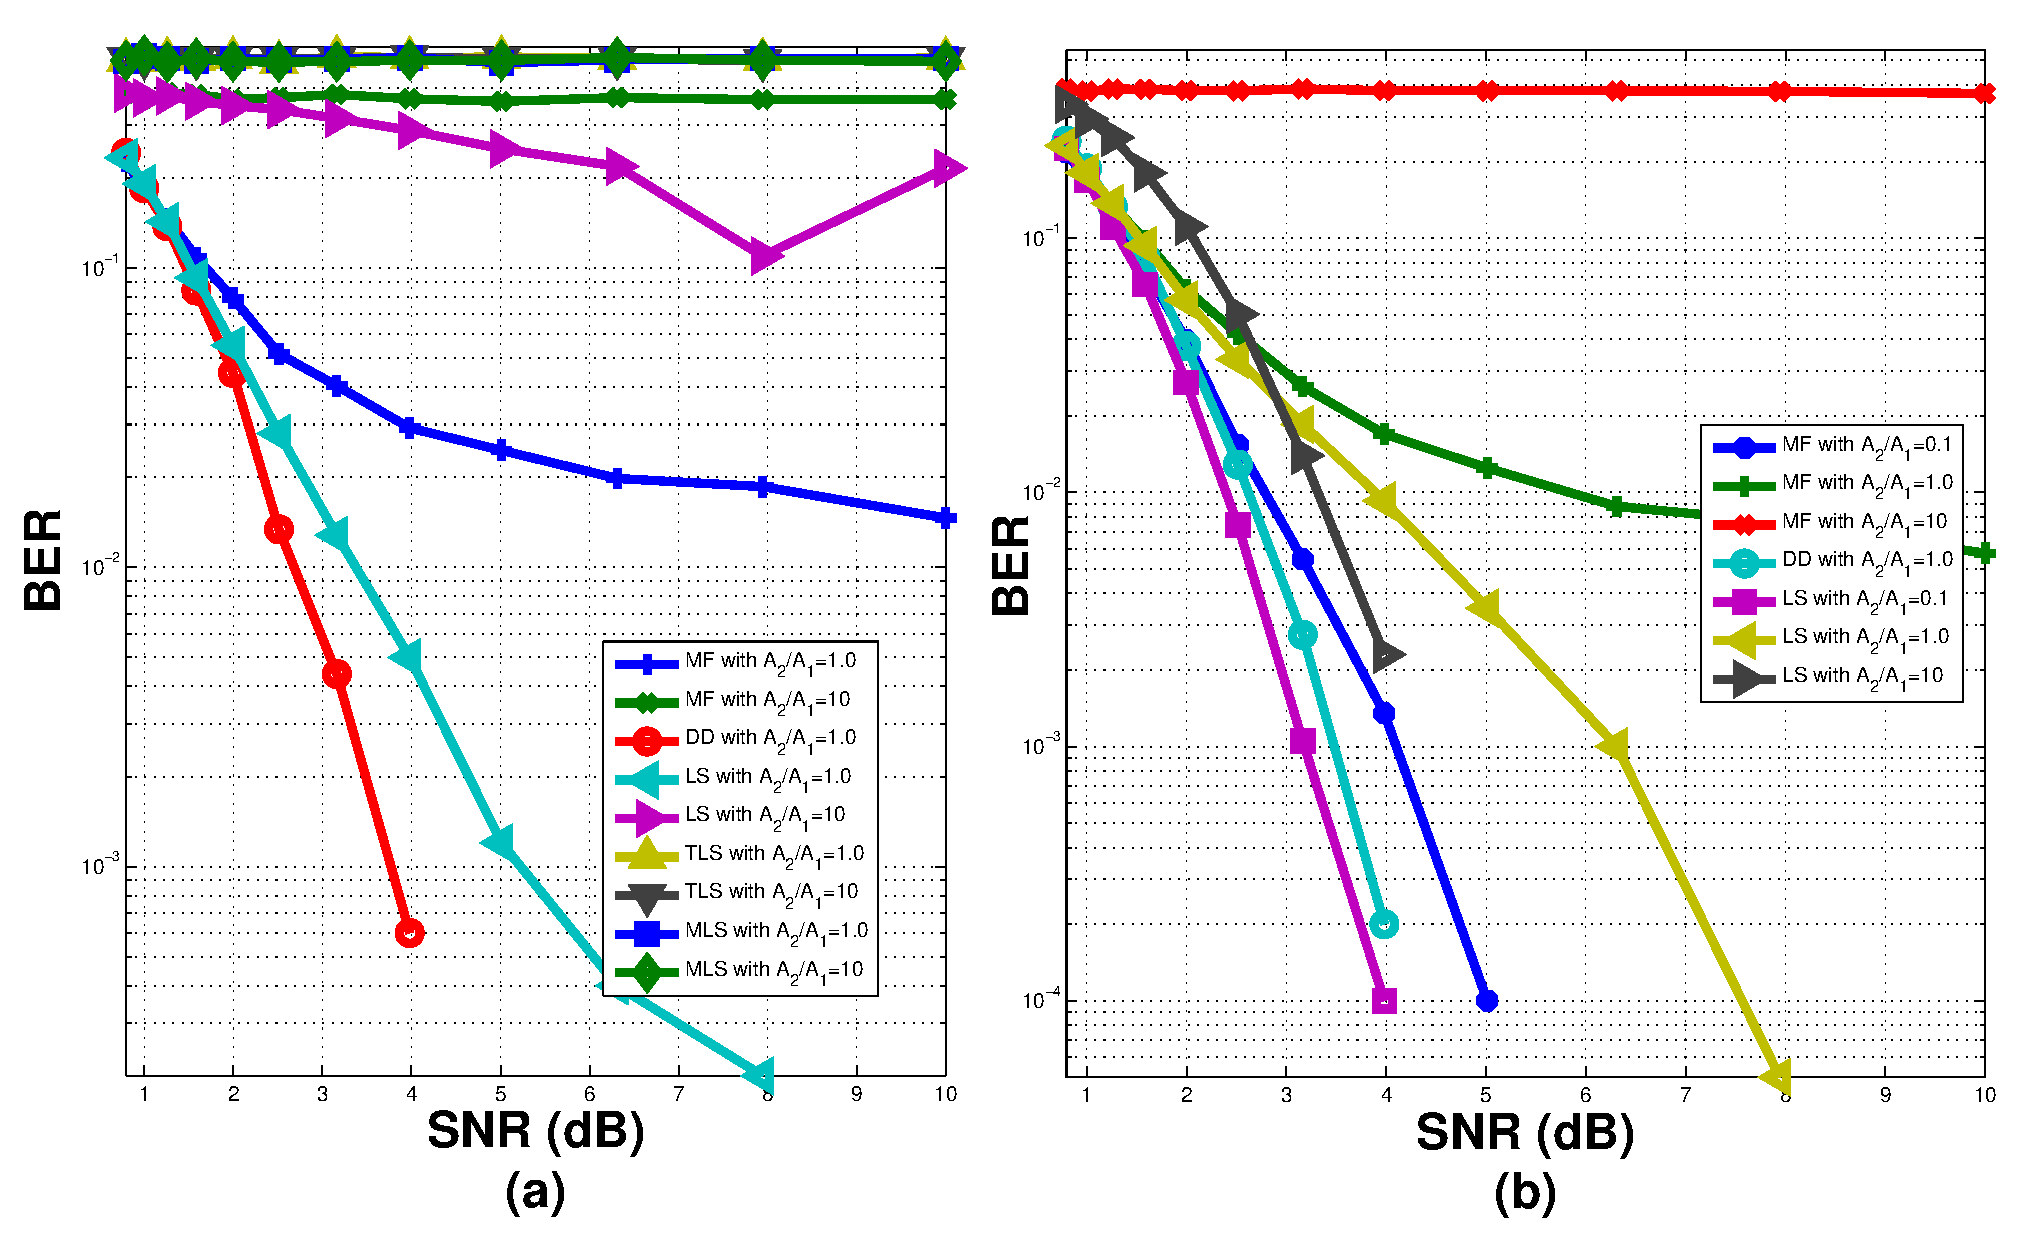
\includegraphics[width=3in]{BER_SNR_10_64.eps}
\caption{ (a) The performance of the proposed blind MUDs against
SNR, $M=12$. (b) The performance of the proposed blind LS
detector, $M=63$. } }\label{BER_SNR}
\end{figure}
\begin{figure} \center{
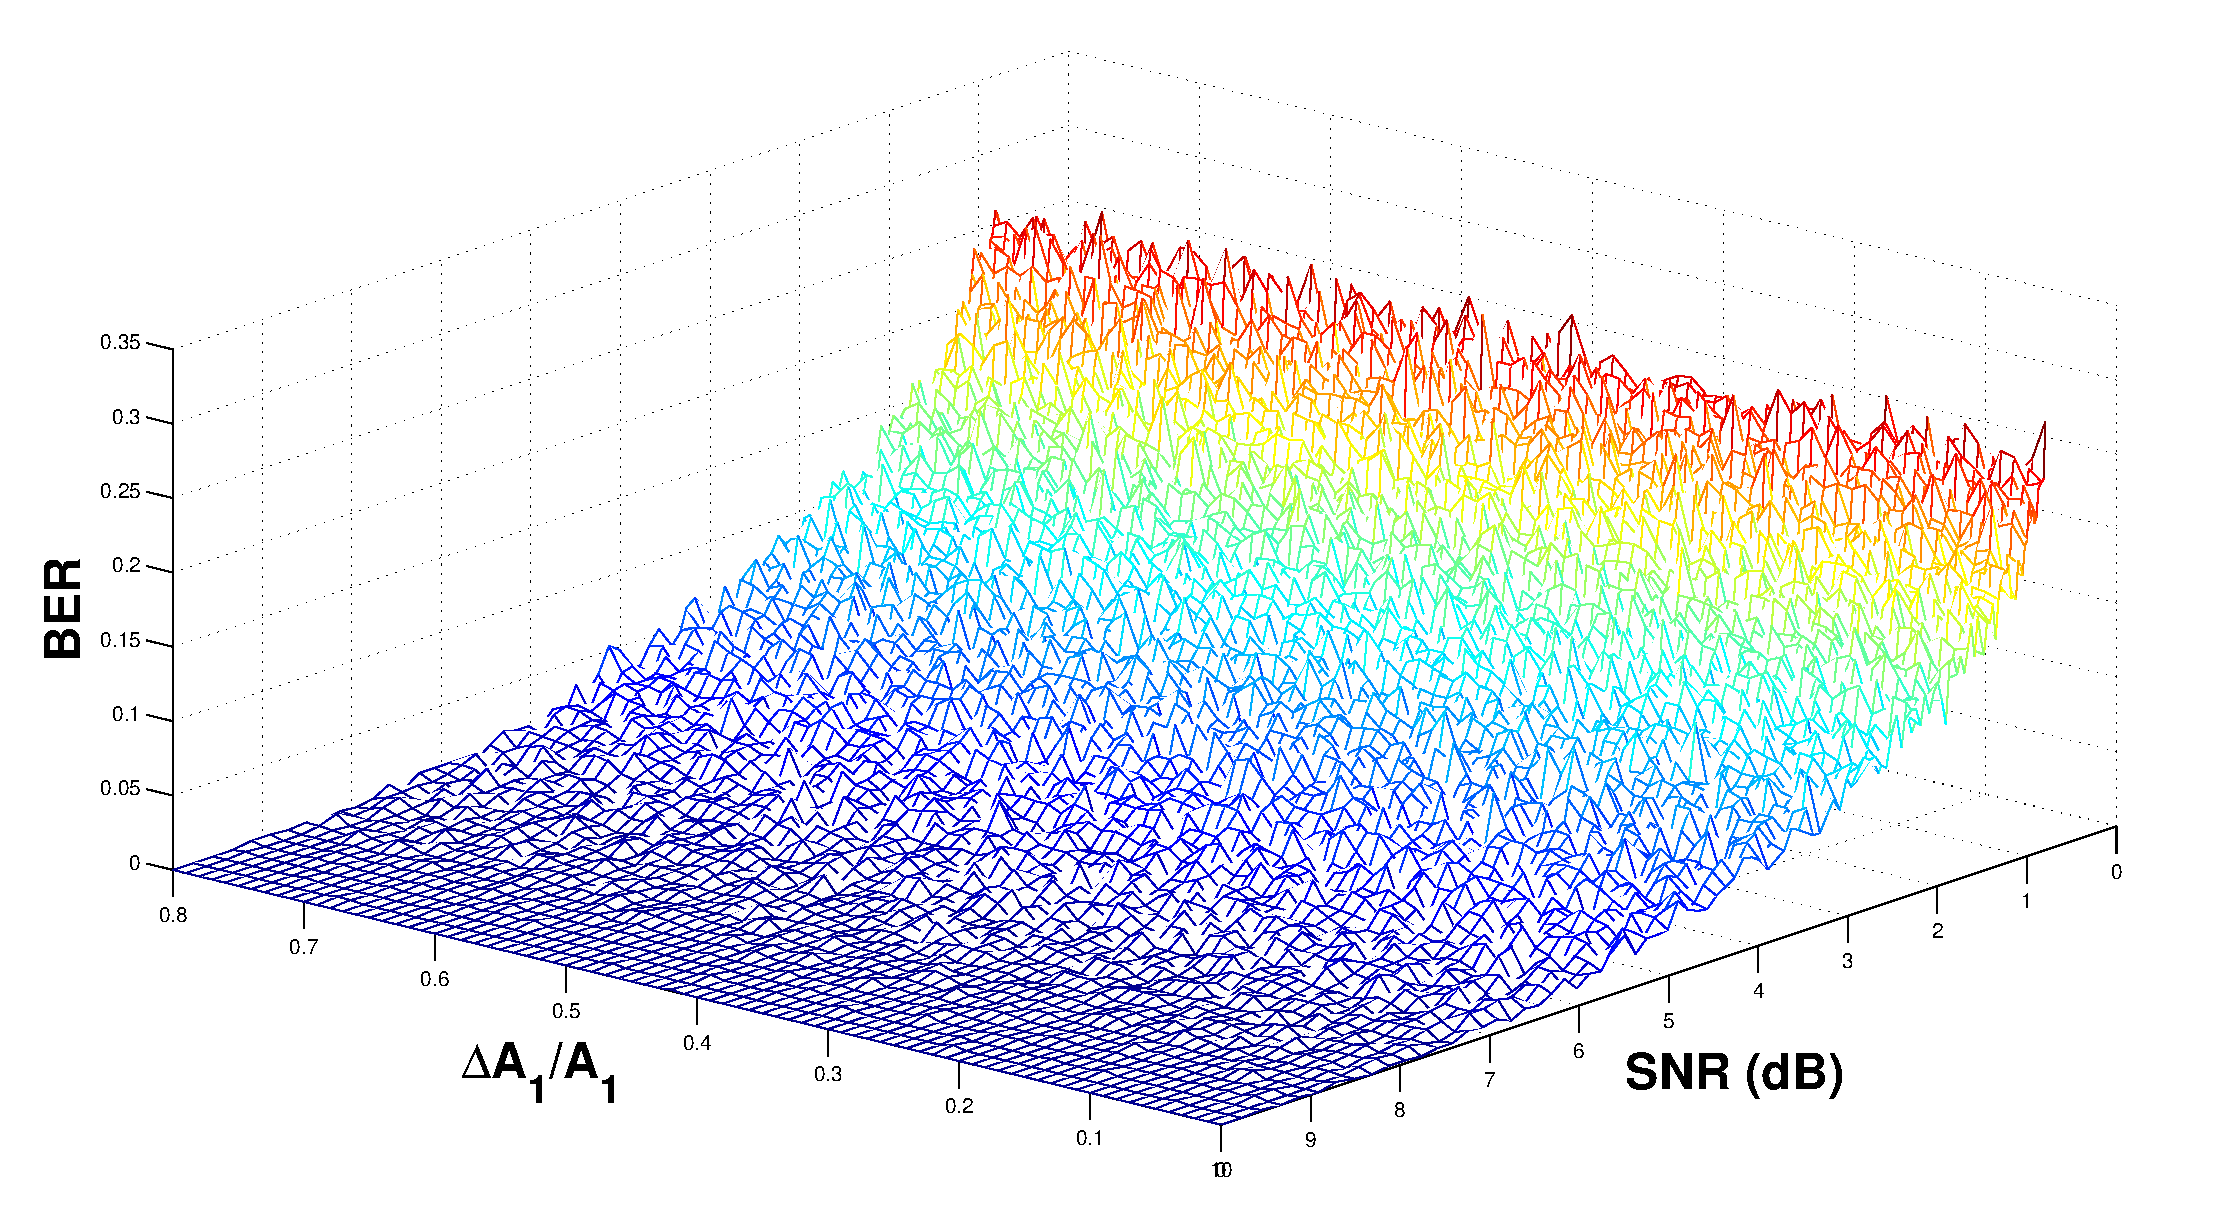
\includegraphics[width=2.5in]{BER_A_SNR_10_64_LSs.eps}
\caption{ The performance of the LS detector against amplitude
estimation error ${\Delta}{A_1}/A_1$ and SNR, $M=63$.}
}\label{BER_A_SNR}
\end{figure}
\begin{figure}
\center{
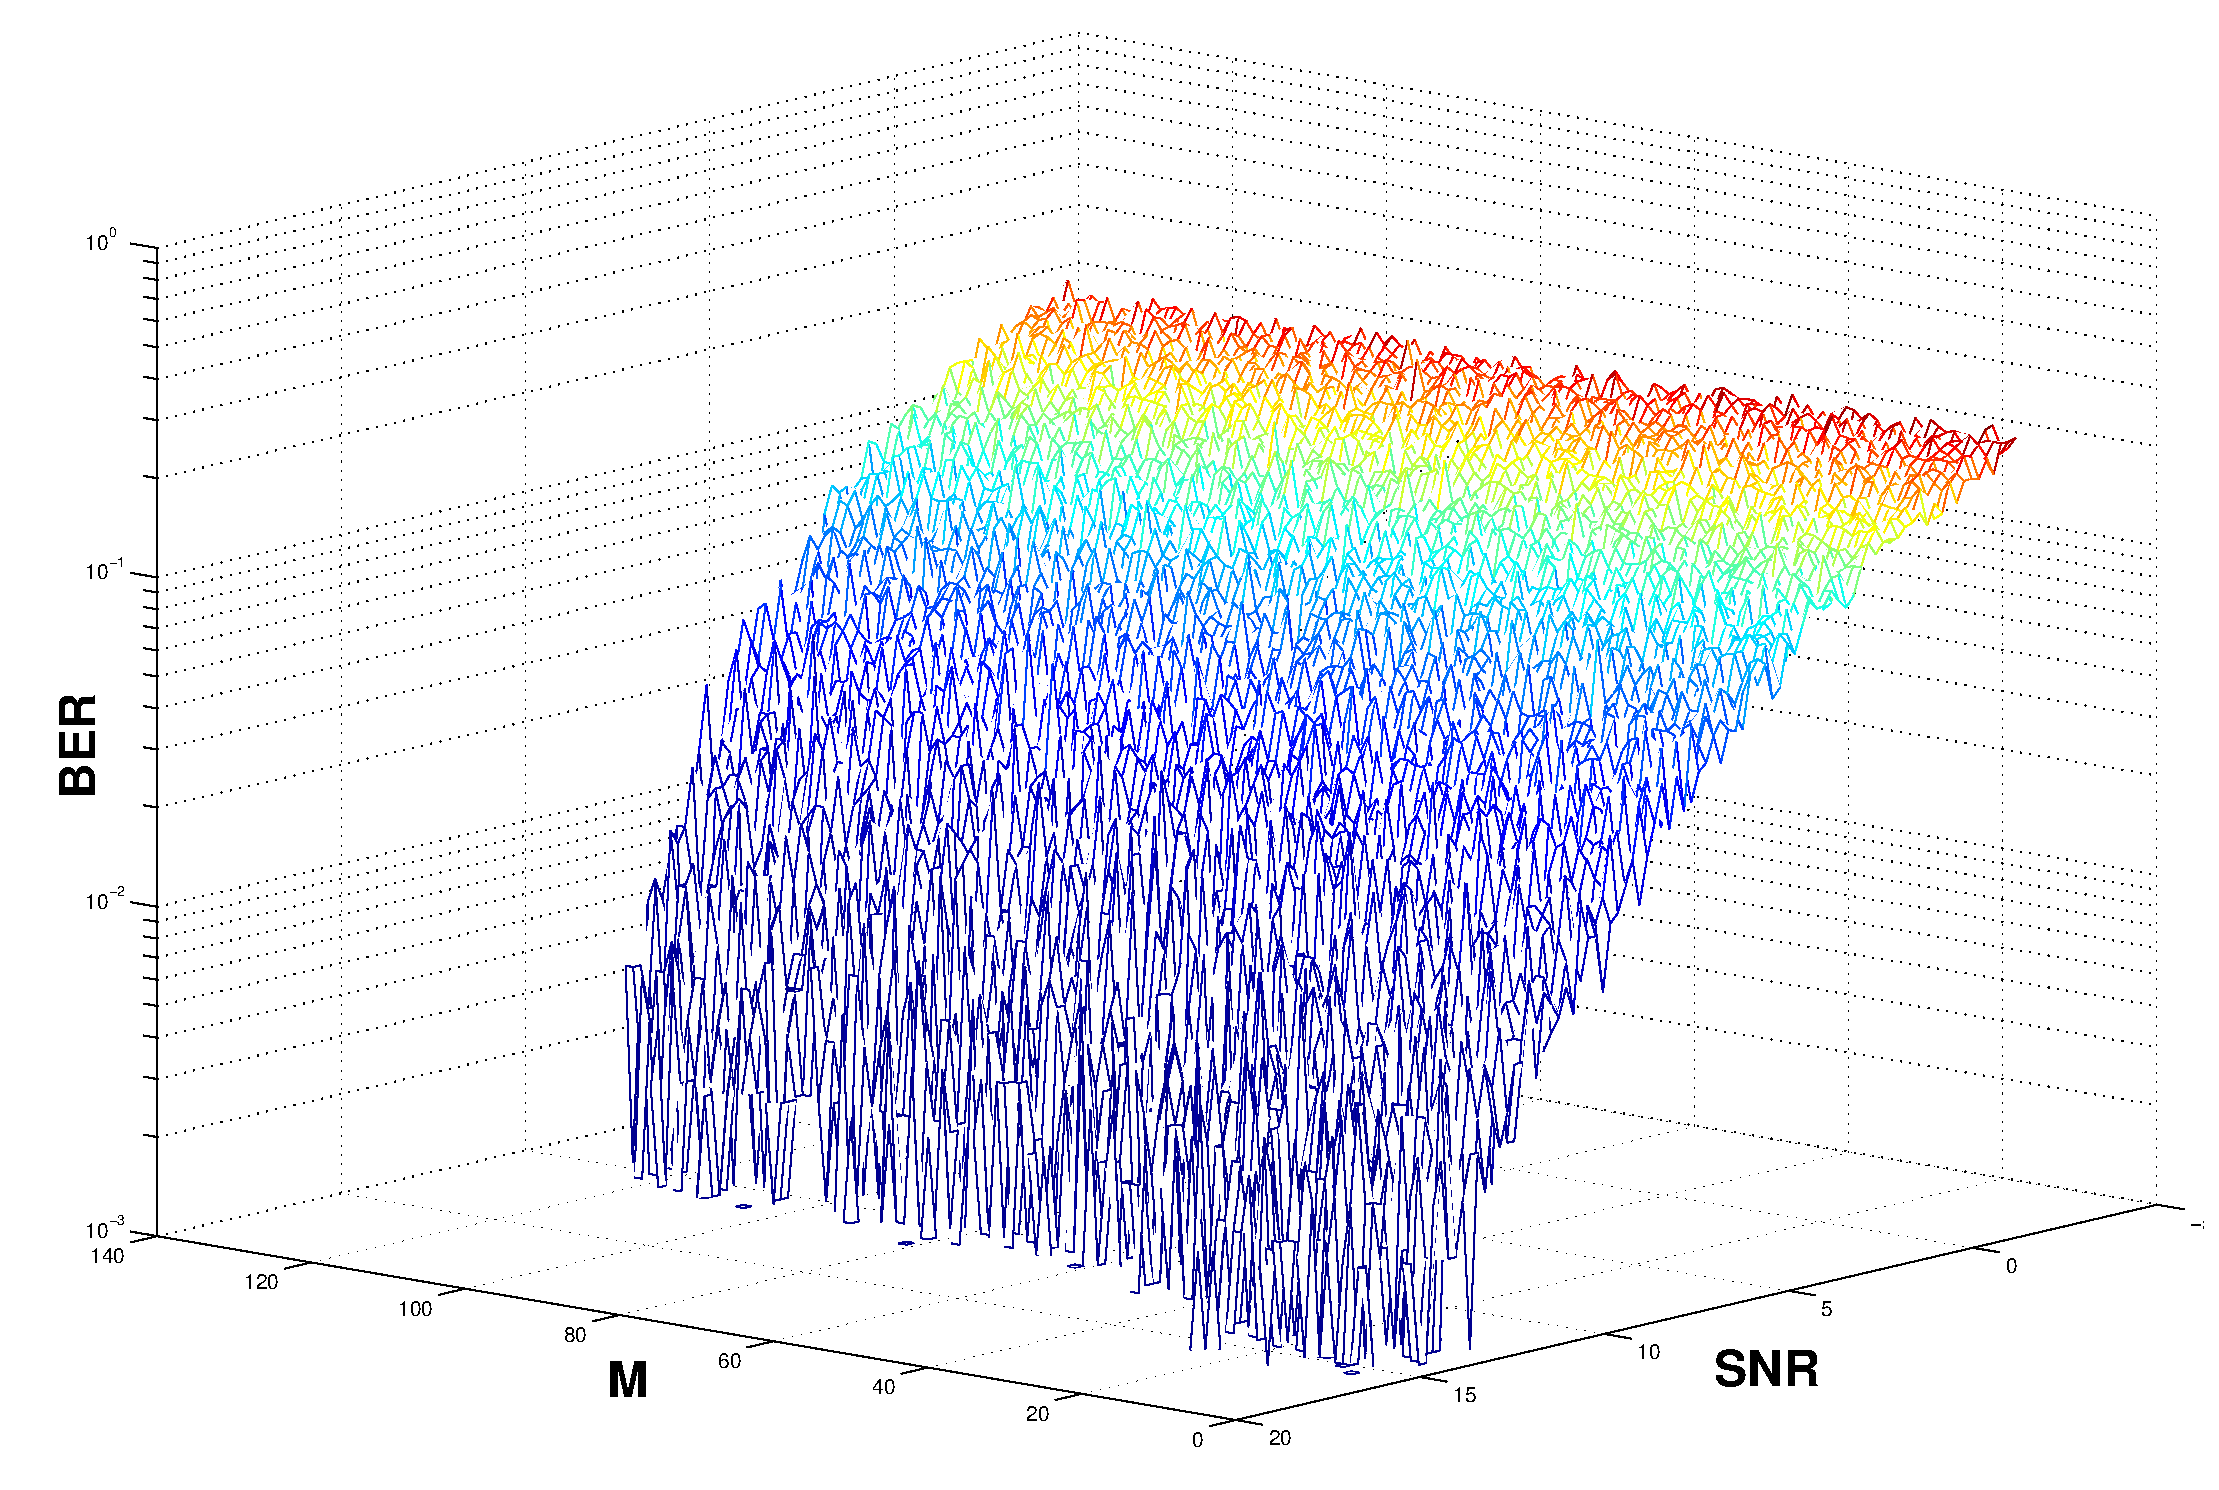
\includegraphics[width=2.5in]{BER_M_SNR_10_64_LSs.eps}
\caption{ The performance of the LS blind MUD against $M$ and
SNR.} }\label{BER_M_SNR}
\end{figure}
\section{Conclusions}
In this paper, we proposed a blind multiuser detection framework
as well as several blind detectors. The proposed blind detectors
are direct and simple without any channel or spreading sequence
estimation or subspace separation operation.

\small
\bibliographystyle{unsrt}
\bibliography{FastBDD,InterferenceCancellation}
\end{document}
